\documentclass[Main.tex]{subfiles} 
\begin{document}

\subsubsection{Use Case 1: Vis busruter}

Vis busruter Use Casen, er den f�rste Use Case, brugeren kan starte, i TrackABus mobil applikationen. Hvis brugeren har installeret en hel ny kopi af applikationen, er denne Use Case den eneste han kan starte. Den starter n�r man trykker p� "View busroutes"-knappen fra hovedsk�rmen. Ved dette tryk startes BusListMenuActivity. I OnCreate s�ttes der en progressbar, som k�rer indtil processen er f�rdig, herefter g�r kaldes onCreate(), som unders�ger om der internettet kan tilg�s. Hvis ikke, f�rdigg�res progressbaren og brugeren notificeres om, at der ikke kunne skabes forbindelse til nettet. Hvis der derimod er net,  tilg�s TrackABusProvideren som en BoundService og rutenumrene bliver hentet. Alle funktioner i servicen sker i en seperat tr�d, og svarer tilbage til viewet via en MessageHandler. N�r rutenumrene er hentet, sender TrackABusProvideren en besked til den medsendte MessageHandler, som er oprettet i BusListMenuActivity. Hvis ingen ruter blev fundet, notificeres brugeren om dette og progresbaren f�rdigg�res. Ellers oprettes der en ListBusData for hver rute, og hvis nummeret eksisterer i SQLite databasen s�ttes denne rute som en favorit i listen. En BusListAdapter oprettes, og samtlige oprettede ListBusData s�ttes i den. P� det simple sekvens diagram, kan hovedforl�bet for denne Use Case f�lges. Efter denne Use Case er fuldendt, kan Use Case 2 og 4 tilg�s. Hvis Use Case 4 i forvejen er gennemg�et, kan Use Case 2 startes fra hovedsk�rmen. P� figur \ref{fig:UC1SSD} kan et sekvensdiagram over forl�bet ses\\\\

\begin{figure}[h!]
\centering
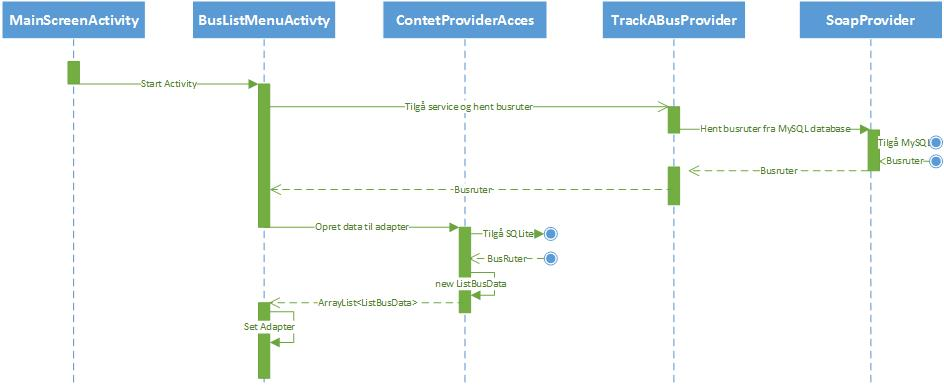
\includegraphics[scale=0.60]{Diagrammer/Sekvensdiagrammer/UC1SSD.jpg}
\caption{Sekvensdiagram over Use Case 1}
\label{fig:UC1SSD}
\end{figure}
\newpage
\end{document}